\section[Operating system concepts]{Operating system concepts}

In this section, we will revise some concepts of OS on multiprogramming system. Multiprogramming defines a computer where it can run several programs simultaneously. To enable multiprogramming, the OS must be capable of managing memory region for processes, scheduling running time for processes, and many more crucial tasks. We will briefly review the two aspects of multiprogramming.

\subsection[Scheduling]{Scheduling}

The first aspect of reviewing is scheduling. Cooperative multitasking, or so-called non-preemptive multitasking, is a design for multiprogramming scheduling where it does not limit a process's runtime. A process will actively run until it stops/idles or waits for an I/O operation, whence the operating system will change (switch context) to another process. In contrast with cooperative multitasking, preemptive multitasking limits the process's runtime and initiate a context switch when either the time allotted is used or the process waits for an I/O operation, Figure~\ref{fig:preemptive}. Both schemes have been used in many operating systems. However, cooperative multitasking schema is not suitable for a multitasking OS, and thus in modern operating systems for general usage (Windows, macOS, and most Linux distributions), preemptive multitasking schema is chosen.

\begin{figure}[h]
  \centering
  \caption{Preemptive scheme}
  \label{fig:preemptive}
  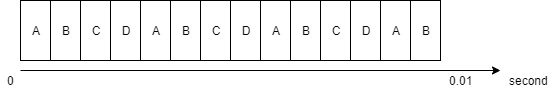
\includegraphics[scale=0.4]{images/preemptive.png}
\end{figure}

\subsection[Memory management]{Memory management}

The second aspect of OS in discusses is memory management. In the early days, memory management was so simple that it would contain the whole process consecutively in memory. However, doing this leads to external fragmentation, where the memory is empty but not fit consecutively for a process, Figure~\ref{fig:externalfragmentation}. OS developers soon realized storing the whole process in memory is not optimize when programs only need a part of memory at a specific time when running. They came up with ways to load only the necessary parts in memory. After many years, people have agreed upon splitting a process to equal parts called a \textit{page}. The OS splits the physical memory to pages and load processes data to those pages, Figure~\ref{fig:splitprocess}. When a process needs more space or needs parts that are not on the memory, the OS will find an empty/unused page to load in. If there is no empty page, one least use page will be moved (swapped out or page out) to disk to make space. The OS tracks what pages a process is using and swap those pages in and out by process need.

\begin{figure}[H]
\centering
\caption{External fragmentation}
\label{fig:externalfragmentation}
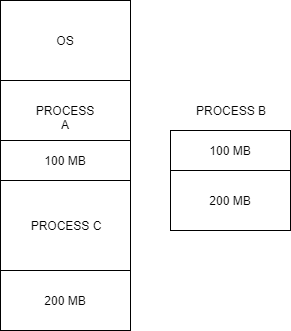
\includegraphics[scale=0.5]{images/external_fragmentation.png}
\end{figure}

So far, we have only discussed processes that have a limited amount of memory, but the OS allows programs to have more space by using the paging technique describe above. Because process data can be moved to disk and brought back when needed, a process can have as many spaces as the disk space available. However, by most OS implementation, a process should have a limited virtual address space. Because the address is virtual to the process, every memory access will need the OS to change to the address in the physical memory (after page swapping). Changing address from virtual to physical is called \textit{address translation}. By using virtual memory, the OS can map the same data to many processes and reuse data. For example, two processes use the same library in Figure~\ref{fig:samelib}.

\begin{figure}[H]
\centering
\caption{Splitting process}
\label{fig:splitprocess}
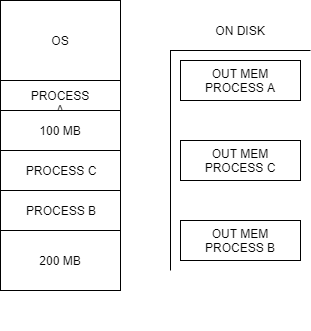
\includegraphics[scale=0.5]{images/splitting_process.png}
\end{figure}

Example of an address translation. Assuming the OS allows a process to have 2GB of (virtual) memory space (from 0 to $2^{32}-1$), and a page will have the size of 4KB, and the system has 4GB of physical memory. A process loading at 0x40000000 will have all data from 0x40000000 to (0x40000000 + 4KB) loaded to physical memory at the address of 0x60000000 to (0x60000000 + 4KB).

\begin{figure}[H]
\centering
\caption{Two processes use the same library}
\label{fig:samelib}
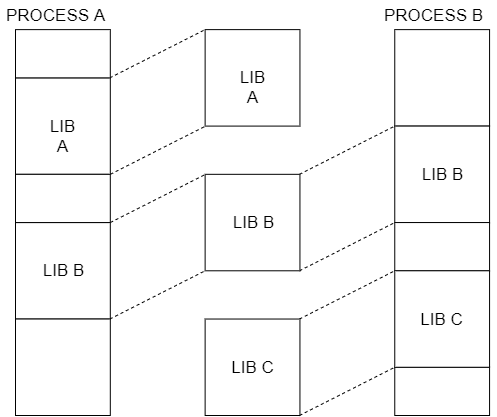
\includegraphics[scale=0.5]{images/use_same_lib.png}
\end{figure}
